\documentclass{article}
\usepackage[latin1]{inputenc} 
\usepackage[T1]{fontenc}
\usepackage{url}
\usepackage[margin=3cm]{geometry}
\usepackage{verbatim}
\usepackage[francais]{babel}

\title{INFO-H303 - Projet - Partie 1}
\author{Wets Loukas, Alfaro Perez Victor, Muller No�mie}


\begin{document}
\maketitle

\renewcommand{\abstractname}{}

\begin{abstract}
TEST BLABLABLA
\end{abstract}

\section{Mod�le entit�-association}
Ins�rer class-diagram ici (mod�lisant le projet et ses contraintes)

\iffalse
\begin{figure}[hb]
\begin{center}
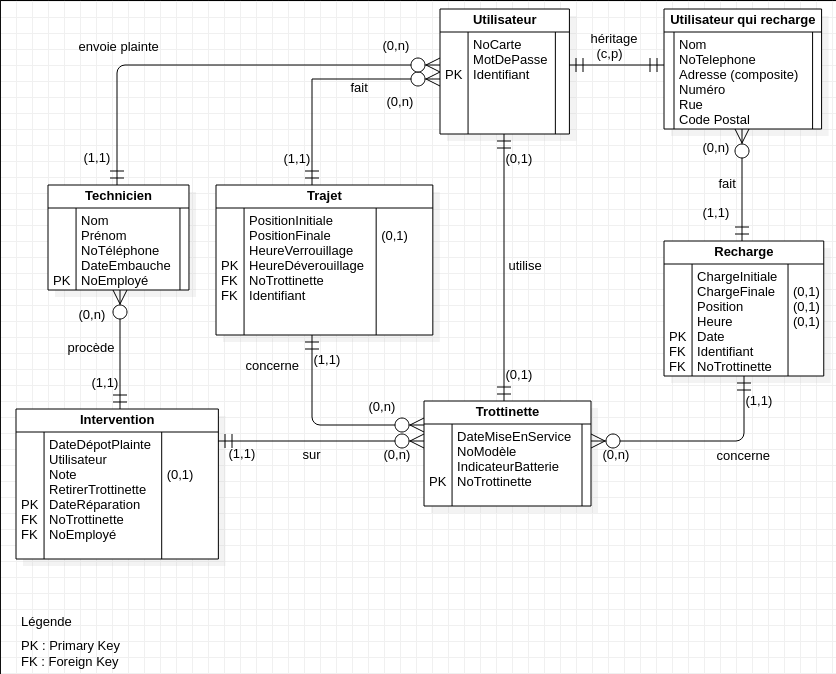
\includegraphics[scale=0.4]{image.png} 
\end{center}
\caption{Mod�le entit�-association}
\end{figure}
\fi 

\subsection*{Contraintes d'int�grit�}

Doivent �tre exprim�es en fran�ais ou anglais et utiliser les m�mes noms d'entit�s, d'associations ou d'attributs que dans le mod�le conceptuel.

\subsection*{Remarques}
Exprimer et justi??fier des hypoth�ses sur le mod�le

\section{Mod�le Relationnel}
A d�duire du mod�le entit�-association, traduction relationnelle du diagramme et de ses contraintes

\subsection*{Contraintes}
[...]

\subsection*{Remarques}
Justifier les choix de mod�lisation

Les deux mod�les doivent servir de support aux requ�tes suivantes :
R1 : La liste et la localisation des trottinettes actuellement disponibles.
R2 : La liste des utilisateurs ayant utilis� toutes les trottinettes qu'ils ont recharg�es.
R3 : La trottinette ayant eeffectu� la plus grande distance.
R4 : Les trottinettes ayant d�j� fait l'objet d'au moins une dizaine de plaintes.
R5 : Les utilisateurs ayant d�j� r�alis� au moins 10 trajets avec pour chaque utilisateur concern� : la dur�e moyenne de ses trajets en trottinette, le nombre total de trajets r�alis�s, le montant total d�pens� en trajets (sans prise en compte de l'argent gagn� par les recharges �ventuelles de trottinettes).





\end{document}
